\documentclass[screen, aspectratio=43]{beamer}
\usepackage[T1]{fontenc}
\usepackage[utf8]{inputenc}

% Use the NTNU-temaet for beamer 
% \usetheme[style=ntnu|simple|vertical|horizontal, 
%     language=bm|nn|en, 
%     smalltitle, 
%     city=all|trondheim|alesund|gjovik]{ntnu2017}
\usetheme[style=ntnu,language=en]{ntnu2017}

\usepackage[english]{babel}
\usepackage[style=numeric,backend=biber,natbib=false,sorting=none]{biblatex}

\title[AP-intro]{MCT4048: Audio Programming}
\subtitle{The Fundamentals: Graphical User Interfaces}
\author[A. Xamb{\'o}]{Anna Xamb{\'o}}
\institute[NTNU]{Department of Music, NTNU}
\date{8 February 2019}
%\date{} % To have an empty date

\addbibresource{../ap.bib} % Add bibliography database

% Set the reference style to numeric.
% See here: http://tex.stackexchange.com/questions/68080/beamer-bibliography-icon
\setbeamertemplate{bibliography item}[text] 

% Set bibliography fonts to a small size.
\renewcommand*{\bibfont}{\footnotesize}

\begin{document}

\begin{frame}
  \titlepage
\end{frame}

% Alternatively, special title page command to get a different background
% \ntnutitlepage
%
\begin{frame}
\frametitle{Assignment 1: Presentation WAC paper (individual)}

Present a summary of a WAC paper of your choice to the class.\\ 
The presentation should last 5 min + 1 min for questions.

\vspace{10 mm}

Schedule of presentations 8.2.19:
\begin{itemize}
\item Karolina
\item Mari
\item Sam
\item Sepehr
\item Shreejay
\end{itemize}
\end{frame}
%
\begin{frame}
\frametitle{This Week: The Fundamentals (40\% Individual Work)}
\begin{itemize}
\item \textbf{Syllabus}: \url{https://uio.instructure.com/courses/17406}
\item \textbf{Assignment 1} (Total grade: 10\%): Presentation WAC paper (individual) -- \textcolor{olive}{day 3 (February 7, 2019)} or \textbf{\textcolor{olive}{4 (February 8, 2019)}}
\item \textbf{Assignment 2} (Total grade: 20\%): Presentation mini-project 1 (individual) -- \textcolor{olive}{days 2 (February 6, 2019) (5\%)}, \textcolor{olive}{3 (February 7, 2019) (5\%)}, \textbf{\textcolor{olive}{4 (February 8, 2019) (10\%)}}
\item \textbf{Assignment 3} (Total grade: 10\%): Written blog post about the mini-project 1 -- February 11, 2019
\end{itemize}
\end{frame}
%
\begin{frame}
\frametitle{Program: Day 4 -- 8 February, 2019}
\begin{itemize}
\item 9.15-10.30: WAC paper presentations (2/2)
\item 10.30-11.00: Setting up computers with the tools for the tutorial
\item 11.00-12.30: Tutorial: Graphical User Interfaces
\item 12.30-13.00: Lunch break
\item 13:00-15:00: Mini-project 1 development (4/4)
\item 15.00-16.00: Final presentations mini-project 1 (3/3)
\end{itemize}
\end{frame}
%
\begin{frame}
\frametitle{Learning Outcomes}
\begin{itemize}
\item Get familiar with how to improve the look-and-feel of web-based projects using CSS files.
\item Be capable of improving the design of web audio interfaces using external libraries and CSS files.
\item Be able to create an independent project relating concepts and building up from previous knowledge.
\item Be aware of best practices in web development of own projects.
\end{itemize}
\end{frame}
%
\begin{frame}
\frametitle{Start setting up...}
Download: \url{https://github.com/axambo/audio-programming-workshop/} 
\\
\vspace{10 mm}
Go to: \texttt{code/d4/}
\end{frame}
%	
\begin{frame}
\frametitle{Debugging JavaScript}
 \texttt{debugger;}\\
 \texttt{breakpoints;} 
\end{frame}
%
\begin{frame}
\frametitle{Functions in JavaScript}
\texttt{x = sum (1, 2);}\\
\vspace{10 mm}
\texttt{function sum (a, b) \{}\\
\setlength\parindent{24pt} \texttt{return a + b;}\\
\setlength\parindent{0pt}\texttt{\}}
\end{frame}
%
\begin{frame}
\frametitle{The Three Legs}
   \begin{figure}
	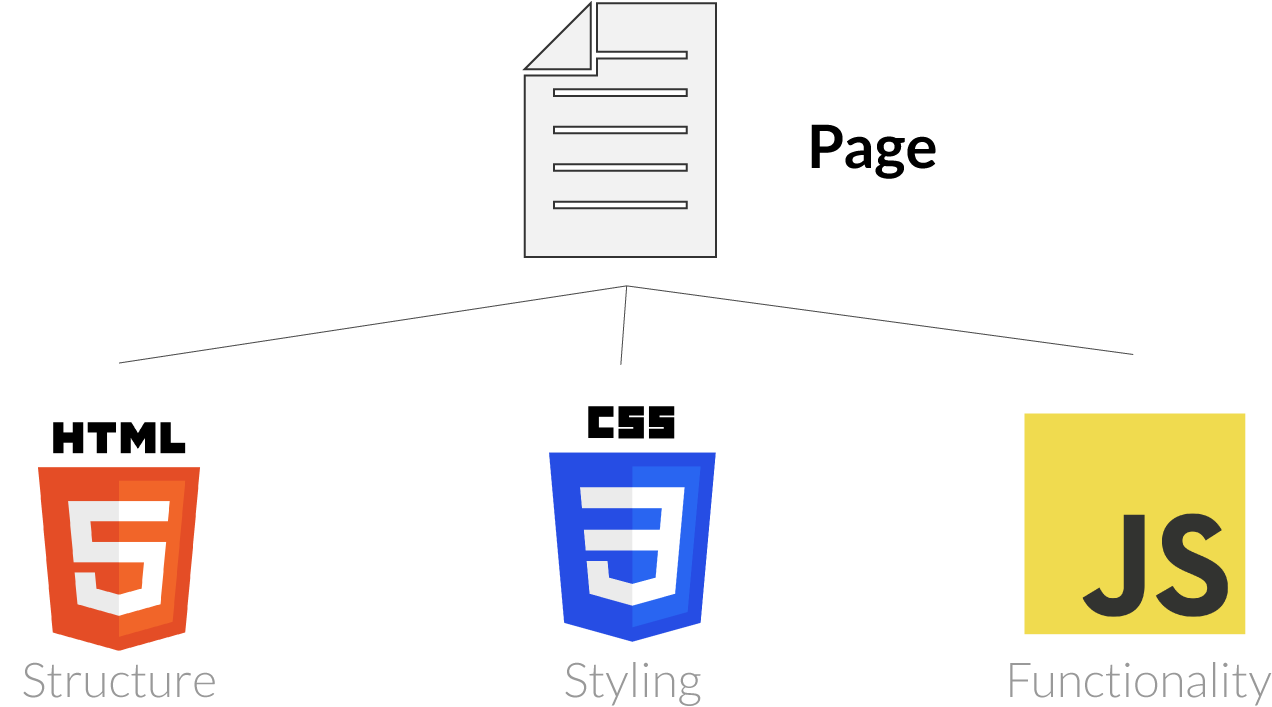
\includegraphics[scale=0.2]{img/three-legs-codeanalogies-blog.png}
    \end{figure}
\vspace{10 mm}
\center{\tiny{Image source: blog.codeanalogies.com}}    
\end{frame}
%
\begin{frame}
\frametitle{CSS}
\begin{itemize}
\item Cascading Style Sheets are used for styling web applications.
\item CSS files use the .css file extension.
\item To connect the CSS with an HTML file, you must link the file from the HTML document using the \texttt{<link>} element in the \texttt{<head>}.
\end{itemize} 
\end{frame}
%
%\begin{frame}
%\frametitle{JSON}
%\begin{itemize}
%\item 
%\end{itemize} 
%\end{frame}
%
\begin{frame}
\frametitle{NexusUI.js}
\begin{itemize}
\item NexusUI.js is a collection of HTML5 interfaces and JavaScript that is helpful for building web audio interfaces.
\item The collection includes buttons, dials, sliders, toggles, and so on.
\item It is possible to change the colors and look-and-feel (\texttt{.colorize()}, CSS).
\end{itemize} 
\end{frame}
%
\begin{frame}
\frametitle{Mini-project development (4/4)}
You are expected to create a mini-project that should be doable within a week. The overall aim is to get familiar with Web Audio. Here are different approaches that you can take:
\begin{itemize}
\item Develop an idea based on what we are seeing in class. Feel free to build up everyday, or change if not convinced.
\item Adapt an existing code to your needs and document what are the changes.
\item Other?
\end{itemize}
\end{frame}
%
\begin{frame}
\frametitle{Working style}
\begin{itemize}
\item Individual work but in shared rooms. You are encourage to share and discuss with your peers.
\item One-to-one talks via Zoom or personally with the instructor to catch up.
\item There will be 4 time slots during the week to work on the project. It is OK to change the topic over the course of the week. Keep a research journal.
\end{itemize}
\end{frame}
%
\begin{frame}
\frametitle{Assignment 2 (part 3) (10\%) - Final Presentation Mini-Project}
Order provided by the shuffle algorithm :)
Spend 5 min max. explaining the following:
\begin{itemize}
\item \textbf{Description}: What is the title of the project and main concept. Overview of the technologies used.
\item \textbf{Timeline}: Provide an overview of the 3 days that you have been working in the mini-project. What have you been working on?
\item \textbf{Achievements}: Give a summary of the achievements of this week through the project. Any progress?
\item \textbf{Challenges}: Give a summary of the challenges that you have been encountering over the week and how you did face them?
\item \textbf{What is next?} e.g. blog post, code repository, website publishing... more development?
\end{itemize}
\end{frame}
%
\begin{frame}
\frametitle{Assignment 3 (10\%) - Written Blog Post Mini-Project}
\textbf{Deadline}: February 11, 2019
\begin{itemize}
\item Make sure to include the information requested in your presentation (see previous slide) plus feedback received.
\item Be familiar with the new metadata to be used so that the blog post has author name, date, the right category (``Audio-Programming''), and a thumbnail for the homepage. See the documentation at: \url{https://github.com/MCT-master/mct-master.github.io/blob/master/README.md}.
\item At least you should use a screenshot and an embedded video showcasing the mini-project. It is a plus if you add links to the source code and a live link (e,g. directory in a personal webpage).
\item Add relevant links in the text to generate traffic.
\end{itemize}
\end{frame}
%
\begin{frame}
\frametitle{Relevant Links}
\begin{itemize}
\item Syllabus: \url{https://uio.instructure.com/courses/17406/pages/syllabus}
\item GitHub slides \& code: \url{https://github.com/axambo/audio-programming-workshop}
\end{itemize}
\end{frame}
%
%\begin{frame}
%  \frametitle{References}
%  \printbibliography
%\end{frame}
%
\end{document}
